Cette fonction, accessible via le menu Algorithms, permet mettre en évidence les chaînes de bits semblables au même endroit dans un dump.
Elle est accessible en cliquant sur Similarities dans le menu Algorithms. La fenètre suivante apparait alors :

\begin{figure}[!h]
  \begin{center}
  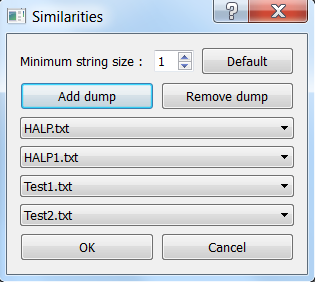
\includegraphics[scale=1]{similaritiesdialog.png}
  \caption{Fenetre de lancement des Similarities}
  \label{similaritiesdialog}
  \end{center}
\end{figure}

L'algorithme est fonctionnel sur 2 dumps, mais comme sur la figure \ref{similaritiesdialog}, il est possible d'ajouter d'autres dumps avec le bouton Add Dump et d'en enlever avec le bouton Remove Dump.
On peut affiner les résultats en entrant une taille minimale de similarité à rechercher, via le paramètre Minimum String Size, ou laisser le logiciel choisir une taille adéquat avec le bouton Default.
Apres avoir valider, l'affichage de la vue text est modifié ainsi :

\begin{figure}[!h]
  \begin{center}
  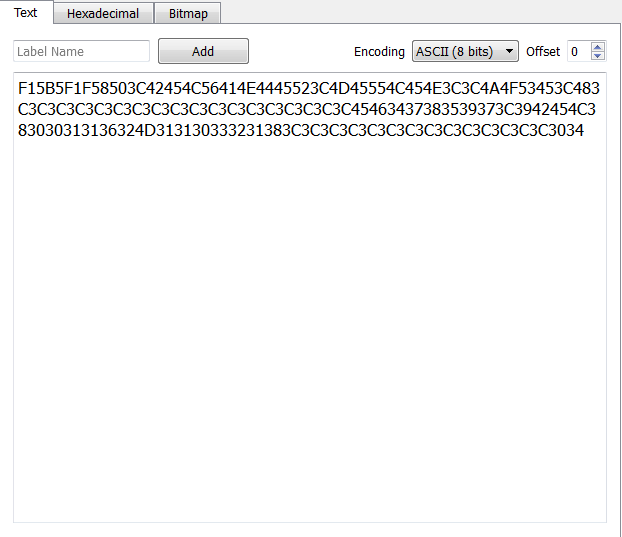
\includegraphics[scale=1]{similaritiescolor.png}
  \caption{Zone text après lancement de l'algorithme de similarities}
  \label{similaritiescolor}
  \end{center}
\end{figure}

Dans le cas de deux dumps, les similarités du dump visualisé sont représentées par la couleur verte, tandis que les dissimilarités du dump visualisé sont représentées par la couleur rouge.
Dans le cas de plusieurs dumps, on dispose d'une troisième couleur, le bleu. Il correspond aux similarités ne concernant pas le dump visualisé (c'est-à-dire les similarités communes à d'autres dumps).
Ces couleurs ont des nuances : plus le vert ou le bleu sont prononcés, plus il y a de dumps partageant la similarité en question.
